\subsubsection{Representaci\'on con compuertas AND, OR y NOT}
\noindent
La representaci\'on de la expresion obtenida previamente mediante compuertas logicas AND, OR y NOT se puede ver a continuaci\'on.

\begin{figure}[h!]
    \centering
    \begin{minipage}{0.85\textwidth}
        \centering
        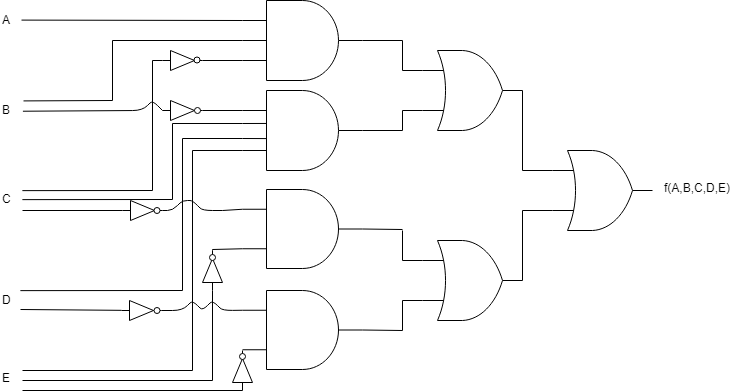
\includegraphics[width=0.9\textwidth]{images/ej2/ej2andornot.png} % first figure itself
         \label{fig:ej2andornot}
    \end{minipage}\hfill
\end{figure}

\subsubsection{Representaci\'on con compuertas NAND}
\noindent
La representaci\'on de la expresi\'on obtenida previamente mediante compuertas logicas NAND se puede ver a continuaci\'on.

\begin{figure}[H]
    \centering
    \begin{minipage}{0.85\textwidth}
        \centering
        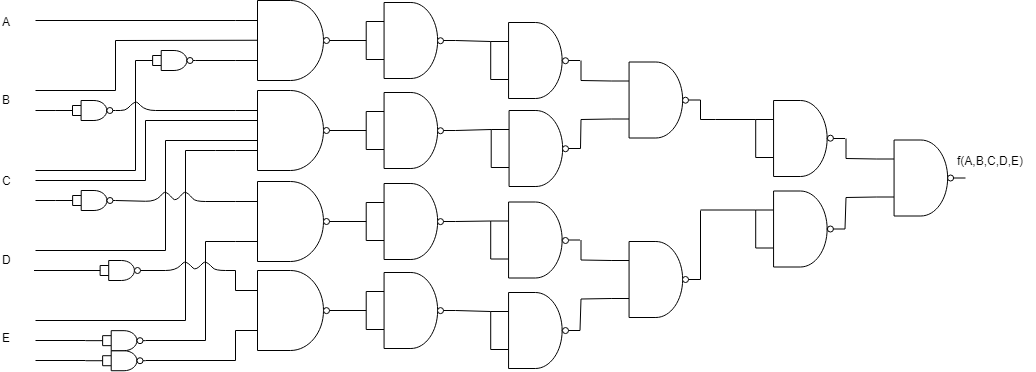
\includegraphics[width=0.9\textwidth]{images/ej2/ej2nand.png} % first figure itself
         \label{fig:ej2nand}
    \end{minipage}\hfill
\end{figure}